\section{Case study: The Array-Based Queueing Lock}
\label{sec:array-lock}

\newcommand{\addition}[1]{\textcolor{red}{ #1 }}

\newcommand{\seq}{\text{seq}}

\renewcommand{\Cap}{\textit{cap}\xspace}
\newcommand{\Rem}{\ensuremath{\;\mathrm{rem}\;}}
\newcommand{\Div}{\ `\text{div}`\ }
\newcommand{\length}{\text{length}\xspace}

\newcommand{\allocN}{\langkw{alloc$_N$}}
\newcommand{\plusl}{+_{l}}

% Multi letter math variables we use
\newcommand{\Array}{\textit{array}\xspace}
\newcommand{\xs}{\textit{xs}\xspace}
\newcommand{\ps}{\textit{ps}\xspace}
\newcommand{\ticket}{\textit{ticket}}
\newcommand{\Next}{\textit{next}}

\newcommand{\lockedGKO}{\text{locked}(\gamma, \kappa, o)}
\newcommand{\isLockA}{\ensuremath{\isLock(\gamma, \iota, \kappa, l, \Cap, R)}\xspace}
\newcommand{\invitation}{\operatorname{invitation}}
\newcommand{\issuedA}{\text{issued}(\gamma, o)}
\newcommand{\rightK}{\ensuremath{\text{right}(\kappa)}\xspace}
\newcommand{\leftK}{\ensuremath{\text{left}(\kappa)}\xspace}
\newcommand{\bothK}{\ensuremath{\text{both}(\kappa)}\xspace}
\newcommand{\nthTrue}{\text{nthTrue}}
\newcommand{\nthTrueCapO}{\text{nthTrue}(\Cap, o \Rem \Cap)}

\renewcommand{\Prop}{\textsf{Prop}}
\renewcommand{\Val}{\text{Val}}
\newcommand{\GN}{\textsf{GhostName}} % GhostName
\newcommand{\replicate}{\operatorname{replicate}}

% Language keywords
\newcommand{\true}{\textsf{true}}
\newcommand{\false}{\textsf{false}}

\newcommand{\arraylock}{array-based queuing lock\xspace}

The array-based queuing lock (ABQL) is a lock closely related to the ticket
lock. The cache behaviour of the ABQL scales better to a large number of threads
at the cost of increased space usage and of only being safe with a bounded
number of concurrent threads. The latter must be modelled when proving safety of
the lock, and hence the ABQL poses unique and interesting challenges to such
efforts.

In this section we describe the \arraylock{} and its implementation in
\proglang. As we have done for the other locks, we then give and prove a
specification which shows that the ABQL is safe, and hence that it satisfies
mutual exclusion.

\subsection{Arrays in \proglang} \label{sec:array}

As the name of the \arraylock{} implies, its implementation relies on arrays. We
therefore first introduce how arrays are supported in \proglang{}.

One may wonder why arrays are necessary, given that we have already seen how
lists can be implemented in \proglang. The key difference is that arrays offer
constant time random-access to elements in the array. In addition to the
performance benefits of this, it also means that reading and writing elements in
an array is an atomic expression.

We need to be able to create arrays of a given size, access elements in an array
at a specific index, and update values at an index in an array. To this end
\proglang{} includes the following syntactic constructs:
\begin{displaymath}
  \begin{array}{lrcl}
    & \binop & \bnfdef{} & \cdots \ALT \plusl
    \\
    \Expr \quad
    & \expr & \bnfdef{} & \cdots
                          \ALT \allocN(e, e)
    \\
    \ECtx\quad
    & E & \bnfdef{}& \cdots
                     \ALT \allocN(E, e)
                     \ALT \allocN(v, E)
    \\
  \end{array}
\end{displaymath}

In order to express that a location $\ell$ points to an array corresponding to a
list $v$, we use the predicate $\ell \pointsto_{*} v$ with the typing rule
\begin{mathpar}
  \infer{\vctx \proves \wtt{\ell}{\Val} \and \vctx \proves \wtt{v}{\mathrm{list}\ \Val}}
  {\vctx \proves \wtt{\ell \pointsto_{*} v}{\Prop}}
\end{mathpar}

If $n$ is a number and $v$ is a value, then $\allocN(n, v)$ represents the
allocation of an array that is $n$ long and which is initialized with the value
$v$ at every index. We use $\replicate(n, v)$ to denote a mathematical list
consisting of the value $v$ repeated $n$ times. The behavior of $\allocN$ is
then captured by the following rule:
\begin{mathpar}
    \inferH{Ht-allocN}
    { }
    { S \proves \hoare{\TRUE}{\allocN(n, v)}{w . \Exists \ell . w = \ell\land \ell \pointsto_{*} \replicate(n, v)}}
\end{mathpar}
To index into an array the $\plusl$ operator is used. If $\ell$ points to the
start of an array then $\ell \plusl i$ is a location pointing to the value of
the $i$'th element, counting from $0$. If $\xs$ is a mathematical list, we use the notation
$xs_{i}$ to denote the $i$'th entry in the list.
\begin{mathpar}
    \inferH{Ht-load-offset}
    { }
    { S \proves
      \hoare{ \ell \pointsto_{*} \xs \ast \xs_i = e }
            { \deref (\ell \plusl i) }
            {v. v = e \land \ell \pointsto_{*} \xs }}
\end{mathpar}
To update an element in an array we use the store operator in combination with
$\plusl$.
\begin{mathpar}
    \inferH{Ht-store-offset}
    { }
    { S \proves \hoare{ \ell \pointsto_{*} \xs \land n < \length(\xs)}{(\ell \plusl n) \gets v}{v. v = \TT \land \ell \pointsto_{*} \xs[n := v] }}
\end{mathpar}
The operator $\plusl$ can be thought of as pointer arithmetic and then this way
of using arrays is similar to how arrays are implemented in many low-level
programming languages. Handling arrays in this manner in Iris has the benefit
that we only need to add $\plusl$ and can reuse the load and store operators in
the context of arrays.

\subsection{The implementation}
\label{sec:arraylock}

Having seen how arrays work, we now describe the ABQL and present an
implementation in \proglang.

The lock consists of a natural number \textit{next} and an array of booleans
\textit{array}. The number represents the next ticket available and the array
contains \False{} at every entry, except for one, which contains \True{}. The
\emph{index} of the \True{} value in the array represents which ticket currently
grants access to the lock.

Constructing an ABQL takes as argument a natural number \Cap{}, specifying the
capacity of the lock. An array of length \Cap{} is then initialized with \True{}
at the first entry and \False{} at all other entries. The natural number which
represents the next ticket is initially set to 0.

To acquire the lock, a ticket is received using \FAA. The primitive \FAA{}
atomically returns the number stored at a location and adds a number to the stored
value. The received ticket, modulo the capacity of the lock, is an index into
the array. By spinning on the value at this index in the array until it becomes
\True{}, the lock is acquired.

To release the lock, the entry corresponding to the ticket from which the lock
was acquired is updated from \True{} to \False. Then, the next index in the
array, modulo \Cap, is set to \True. This signals to the next thread that it can
acquire the lock.

In the implementation we use a triple to represent the lock. We use $(-, -, -)$
as notation for $((-, -), -)$ and abuse notation slightly by letting $\Proj1$,
$\Proj2$, and $\Proj{3}$ denote the projections of a triple denoted in this
manner. The first element in the triple is the array, the second the
\textit{next} number, and the third is the length of the array, which we store
since arrays in \proglang{} do not have a length operation. The implementation
is then:
\begin{align*}
  \langkw{let} \newLock \Cap = \ & \Let \Array = \allocN(\False,\ \Cap) in \\
                                 & (\Array \plusl 0) \gets \True; \\
                                 & (\Array,\ \Ref(0),\ \Cap) \\
  \langkw{let} \acquire\ l =\ &\Let \Next = \Proj2\ l in \\
                                 & \Let \ticket = \FAA\ \Next\ 1 in \\
                                 & \wait l\ \ticket; \\
                                 & \ticket \\
  \langkw{let} \wait l\ t =\ &
                               \Let \Array = \Proj1\ l in \\
                                 & \Let i = t \Rem (\Proj{3}\ l) in \\
                                 & \If \deref (\Array \plusl i) then () \Else (\wait l\ t) \\
  \langkw{let} \release\ l\ o =\ & \Let \Array = \Proj1\ l in \\
                                 & \Let \Cap = \Proj{3}\ l in \\
                                 & \Array \plusl (o \Rem \Cap) \gets \False ; \\
                                 & \Array \plusl (o + 1 \Rem \Cap) \gets \True
\end{align*}

\subsection{The specification}

The specification can be seen as an extension of the specification for the
ticket lock. The significant changes specific to the ABQL are highlighted in red
in the presentation below.
\begin{align*}
  & \exists \isLock : \GN \to \GN \to \GN \to Val \to \nat \to \Prop \to \Prop. \\
  & \exists \locked : \GN \to \GN \to \Prop. \\
  & \exists \issued : \GN \to \nat \to \Prop. \\
  & \addition{\exists \invitation : \GN \to \nat \to \nat \to \Prop.} \\
  & \quad\quad \forall \gamma, \iota, \kappa, l, \Cap, R.\ \isLockA \Rightarrow \persistently \isLockA \\
  & \color{red} \land\quad \forall \iota, n, m, \Cap.\ \invitation(\iota, n, \Cap) \ast \invitation(\iota, m, \Cap)
       \Leftrightarrow \invitation(\iota, n + m, \Cap) \\
  & \land\quad \forall \Cap, R.\ \hoare{ R \ast \addition{0 < \Cap} }
      { \newLock \addition{\Cap} }
      { l.\ \Exists \gamma, \iota, \kappa. \isLockA \ast \addition{\invitation(\iota, \Cap, \Cap) }} \\
  & \land\quad \forall \gamma, \iota, \kappa, l, \Cap, R.\ \hoare{ \isLockA \ast \addition{\invitation(\iota, 1, \Cap)} }
      { \acquire\ l }
      { \addition{o}.\ \locked(\gamma, \kappa, \addition{o}) \ast R }  \\
  & \land\quad \forall \gamma, \iota, \kappa, l, \Cap, R.\ \hoare{ \isLockA \ast \issued(\gamma, t) }
      { \wait l\ t}
      { \_.\ \locked(\gamma, \kappa, t) \ast R } \\
  & \land\quad \forall \gamma, \iota, \kappa, l, \Cap, R.\ \hoare{ \isLockA \ast \lockedGKO \ast R }
      { \release\ l\ o }
      { \_.\ \addition{\invitation(\iota, 1, \Cap)} }
\end{align*}
The $\isLockA$ predicate represents the knowledge that the value $l$ is a lock
with a capacity of \Cap, and which protects the resource $R$. Since the lock is
supposed to be used in a concurrent setting the \textit{isLock} predicate is
persistent, as we have seen before.
The predicates $\lockedGKO$ and $\issued(\gamma, t)$ serve the same
purpose as they did in the ticket lock.

The precondition for \textit{newLock} requires that a lock must be created with
a capacity greater than zero. This is required as the implementation performs
modulo with \Cap, which is not defined for zero.

The biggest change is the addition of \textit{invitations}. Since every thread
waiting to acquire the lock is spinning on an entry in the array, and since the
array is \Cap long, at most \Cap{} threads may simultaneously attempt to acquire
the lock.

The predicate $\invitation(\iota, n, \Cap)$ denotes the ownership of $n$
invitations where $\Cap$ invitations exists in total. When the lock is created,
$\Cap$ invitations are also constructed, see
the postcondition for $\newLock$. In order to acquire the lock, one invitation
is required and is surrendered to the lock. When a thread later releases the lock, an
invitation is given back, as seen in the postcondition for $\release$, such that
the thread can then acquire the lock again.

Since invitations are not duplicable, we ensure that at most $\Cap$ threads
can simultaneously attempt to acquire the lock. Invitations can be split
and combined, meaning that the ownership of $n + m$ invitations implies the
separate ownership of $n$ and $m$ invitations.

\subsection{Representing invitations with ghost state}

The invitation predicate is implemented as ghost state using the following
resource algebra. We define the carrier of the resource algebra as
\[
  \mathcal{M} = (\nat \times \nat) \cup \bot.
\]
The first number in the pair represents how many invitations are owned, and the
second how many invitations exist in total.

It should not be possible to have more invitations than the total number of
invitations, and hence the valid elements are defined as
\[
\mathcal{V} = \{ (n,m) \mid n \leq m \}.
\]

Since it should be possible to combine and separate invitations, we define the
operation as
\begin{align*}
  (a, n) \cdot (b, m) =
    \begin{cases}
      (a + b, m) & \text{ if } n = m \\
      \bot & \text{ otherwise }
    \end{cases}.
\end{align*}
It only makes sense to combine invitations with the same upper bound, and hence
the operation returns $\bot$ if the two upper bounds are not equal. Invitations
should not be duplicable, and to this end the core function is
always undefined.

With this resource algebra in place, we now define invitations as
\[
  \invitation(\gamma, a, n) = \ownGhost{\gamma}{(a, n)}.
\]

\begin{exercise}
  Show that the resource algebra defined above satisfies the requirements
  given in the definition of a resource algebra
  (Definition~\ref{def:resource-algebra}).
\end{exercise}


\subsection{Implementation of the specification}
\label{sec:implementation-spec}

Having understood the purpose of invitations we are now ready to show that the
implementation meets the specification. We adopt the notation $\seq(o, i)$ for the
set of numbers $\{ n \in \nat \mid o \leq n < o + i \}$ and define the following
predicates:
\begin{align*}
  \isLockA =& \ 
     \Exists a, n, \delta \in \varepsilon. \\
        & \quad l = (a, n, \Cap)\ \ast 0 < \Cap\ \ast \\
        & \quad \knowInv{\delta}{\lockInv(\gamma, \iota, \kappa, a, \Cap, n, R)} \\
  \lockInv(\gamma, \iota, \kappa, a, \Cap, n, R) =& \
    \Exists o, i, xs. \\
        & \quad n \gmapsto (o + i) \ \ast a \gmapsto_{*} xs \ast \length\ \xs = \Cap\ \ast \\
        & \quad \invitation(\iota, i, \Cap) \ast \ownGhost{\gamma}{\authfull ( o, \seq(o, i))} \ast \\
        & \quad \text{state}(\gamma, \kappa, \Cap, o, R, xs) \\
  \text{state}(\gamma, \kappa, \Cap, o, R, xs) =&\ 
        (\ownGhost{\gamma}{\circ (o, \emptyset)} \ast R \ast \bothK \ast xs = \nthTrueCapO) \lor \\
        & \ (\issuedA \ast \rightK \ast xs = \replicate(\false, \Cap)) \lor \\
        & \ (\issuedA \ast \leftK \ast xs = \nthTrueCapO) \\
  \issued(\gamma, t) =&\ \ownGhost{\gamma}{\circ(\munit, \{ t \})} \\
  \lockedGKO =&\ \ownGhost{\gamma}{\circ(o, \emptyset)} \ast \rightK
\end{align*}
In the following subsections we describe these predicates
at a high-level and identify several useful
and central properties as lemmas, which we then refer back to when we present the proofs.
Hopefully this makes it easier for the reader to understand how the various
pieces fit together.

\subsubsection{The ghost state}

The ghost state with ghost name $\gamma$ is defined using the resource algebra
$\authm(\exm(\nat)_{?} \times (\mathbb{P}_{\textit{fin}}(\nat)))$. This is the
same resource algebra used in the ticket lock. Intuitively, an element of this
resource algebra is a pair where the first element can include knowledge about
the value of $o$, which represents that the thread with this ticket currently
has or may acquire the lock, and the second element knowledge about which tickets currently
exist.

We use \emph{disjoint} union such that partial knowledge about the existence
of a ticket can only exist once. Hence we have the following lemma:
\begin{lemma} \label{prop:issuedcontra}
  Only a single thread can know that a certain ticket has been issued.
  \[ \ownGhost{\gamma}{\circ(\munit, \{ t \})} \ast \ownGhost{\gamma}{\circ(\munit, \{ t \})} \wand \bot \]
\end{lemma}
Similarly, the exclusive construct around the value of $o$ ensures that this information can also only exist once.
\begin{lemma} \label{prop:knowocontra}
  Only a single thread can have the partial information about $o$.
  \[ \ownGhost{\gamma}{\circ(o, \emptyset)} \ast \ownGhost{\gamma}{\circ(o, \emptyset)} \wand \bot \]
\end{lemma}

The predicates \textit{left}($\kappa$), \textit{right}($\kappa$), and \textit{both}($\kappa$)
are defined using the
resource algebra $\exm(\unitty)_{?} \times \exm(\unitty)_{?}$ where $\unitty$ denotes
the unit resource algebra with the single element \unittt:
\begin{align*}
    \leftK = \ownGhost{\kappa}{(\unittt, \munit)} \quad \quad
    \rightK = \ownGhost{\kappa}{(\munit, \unittt)} \quad \quad
    \bothK = \ownGhost{\kappa}{(\unittt, \unittt)} .
\end{align*}

\begin{lemma} \label{prop:leftrighcombine}
The resource \bothK splits into \leftK and \rightK, and \leftK and \rightK can be combined back together into \bothK.
\begin{align*}
  \bothK \ \wand \ \leftK \ast \rightK \\
  \leftK \ast \rightK \  \wand \ \bothK
\end{align*}
\end{lemma}
\begin{lemma} \label{prop:bothnocombine} Any other combination of $\leftK$,
  $\rightK$, and $\bothK$ except for those in Lemma~\ref{prop:leftrighcombine}
  is invalid.
\end{lemma}
Both lemmas follow directly from the definition of the resource algebra and the
rules \ruleref{Own-op} and \ruleref{Own-valid}.

\subsubsection{The \textit{isLock} predicate}

The \textit{isLock} predicate states the existence of $a$, which is the array
value, and $n$ which is a location pointing to the index of the next ticket. The
equality $l = (a, n, \Cap)$ describes the physical representation of the lock.
The inequality $ 0 < \Cap $ serves to constrain \Cap such that we can use it to
do division with remainder. Finally, \textit{isLock} contains the invariant
which we describe in the next subsection.

\subsubsection{The invariant}

The invariant \textit{lockInv} states the existence of three things. A natural number $o$,
representing that the thread with this ticket currently has or may acquire the
lock. The number $i$, which represents how many threads are currently waiting to
acquire the lock. Finally, $\xs$ is a list of booleans corresponding to the
current contents of the array.

The invariant contains the points-to predicate for $n$ (from the \textit{isLock} predicate)
\[
  n \gmapsto o + i.
\]
As one would expect, $n$ points to the ticket currently granting access to the
lock added together with the number of threads waiting for the lock.

Inside the invariant we have the authoritative part
\[
  \ownGhost{\gamma}{\authfull ( o, \seq(o, i))}.
\]
The lock always knows the value of $o$ and of all the tickets in existence. Here
we have made an important change compared to the equivalent part in the ticket
lock. In the ticket lock the set of tickets always starts from 0, and it is only
expanded when new tickets are issued. In some sense, tickets are not ``cleaned
up'' after their usage. For the ABQL it is important that the set of tickets
starts at $o$. This means that whenever $o$ increases, we know that all tickets
smaller than $o$ no longer exist. Hence, we have the following lemma.
\begin{lemma} \label{prop:ticketbound}
  From $\issuedA$ and the content of the invariant one can conclude $o \leq t < o + i$.
  More precisely,
  \[
    \ownGhost{\gamma}{\circ(\munit, \{ t \})} \ast \ownGhost{\gamma}{\authfull(o, \seq(o, i)}
    \wand
    \ownGhost{\gamma}{\circ(\munit, \{ t \})} \ast \ownGhost{\gamma}{\authfull(o, \seq(o, i)}
    \ast o \leq t < o + i.
  \]
\end{lemma}
The lemma is straightforward to show. Suppose the two ghost states are owned. By
\ruleref{Own-op} and \ruleref{Own-valid} the product of the two elements of the
resource algebra is also owned and is valid. From the definition of the
authoritative resource algebra and the disjoint set resource algebra this
implies $ \{ t \} \subseteq \seq(o, i) $. Which per the definition of
\textit{seq} means that we have the bound in the lemma. This tighter bound is
not needed for the proofs of the ticket lock to go through but for the ABQL it
is necessary.

The invariant also contains ghost state for invitations, which we have already
described. It is used as \[ \invitation(\iota, i, \Cap) \] inside the invariant.
This establishes the connection that $i$ is the number of invitations owned by
the lock. If $i$ threads are currently waiting for the lock then $i$ invitations
are currently owned by the lock. This corresponds to the specification where,
when calling \textit{acquire}, a thread surrenders an invitation and when
calling \textit{release} the invitation is handed back. In the meantime the
invitation is ``stored'' in the lock. As discussed previously the inclusion of
invitations serves to constrain how many threads can wait for the lock. Indeed
we have the following key property:
\begin{lemma} \label{prop:iLtCap}
The $\invitation(\iota, i, \Cap)$ in the invariant establishes the inequality $i \leq \Cap$.
\[\invitation(\iota, i, \Cap) \wand i \leq \Cap \]
\end{lemma}
This lemma follows from the definition of invitation, \ruleref{Own-valid}, and
the definition of validity of the resource algebra. This lemma is essential when
proving the specification for \textit{wait}.

\subsubsection{The \textit{state} of the lock}

The $\text{state}(\gamma, \kappa, \Cap, o, R, xs)$ disjunction represents the
current state of the lock. The first disjunct corresponds to the lock being
\textit{open} and the disjunct includes resource $R$ since the lock owns the
resource in this state. The last disjunct corresponds to the lock being
\textit{closed}. We call the middle disjunct \textit{clopen}. It is necessary,
since the release function proceeds in \emph{two} atomic steps when it reopens
the lock. Between these two steps the lock is neither closed nor open. Hence
this disjunction is crucial in the proof of release.
\begin{center}
  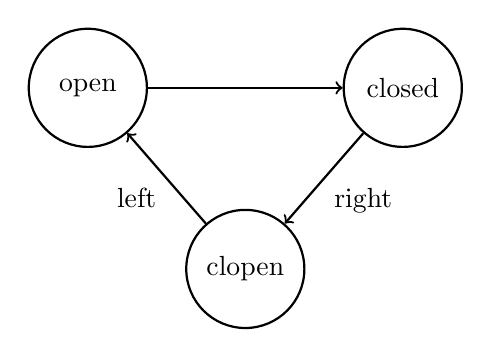
\begin{tikzpicture}[term/.style={circle,draw,minimum size={1.5cm},inner sep=5pt},auto]
    \node [thick] (o) at (0, 0) [term] {open};
    \node [thick] (c) at (4, 0) [term] {closed};
    \node [thick] (cl) at (2,-2.3) [term] {clopen};
    \draw [->,thick] (o) to node {} (c);
    \draw [->,thick] (c) to node {right} (cl);
    \draw [->,thick] (cl) to node {left} (o);
  \end{tikzpicture}
\end{center}
In the first and third disjunct $\nthTrueCapO$ denotes a mathematical sequence
of booleans of length \Cap with \False{} at every index except for index $o
\Rem \Cap$ which contains \True.

\subsubsection{The \textit{issued} token}

The $\issued(\gamma, t)$ token represents the information that the ticket $t$
has been issued. The key property of this token is that if the resource
$\issuedA$ is owned then it is possible to conclude that the lock is open.
\begin{lemma} \label{prop:issuedopen}
  Owning $\issuedA$ is sufficient to conclude that the lock is open.
  \[
\issuedA \ast \text{state}(\gamma, \kappa, \Cap, o, R, xs) \wand
        (\ownGhost{\gamma}{\circ (o, \emptyset)} \ast R \ast \bothK \ast xs = \nthTrueCapO)
  \]
\end{lemma}
This follows since $\issuedA$ is incompatible with itself per
Lemma~\ref{prop:issuedcontra} which leads to a contradiction in the
\textit{clopen} and \textit{closed} branch of the \textit{state} disjunction.

\subsubsection{The \textit{locked} predicate}

The $\lockedGKO$ predicate represents the knowledge that the lock is currently locked
along with the knowledge of what $o$ actually is. The ghost state \rightK is
included such that it is possible to conclude that the lock is in the
\textit{locked} state. This holds since the \textit{open} state contains
$\bothK$ and the \textit{clopen} state contains \rightK, both of which
contradicts with $\rightK$ per Lemma~\ref{prop:bothnocombine}.
\begin{lemma}
  From $\lockedGKO$ it is possible to conclude that the lock is closed.
  \[
    \lockedGKO \ast \text{state}(\gamma, \kappa, \Cap, o, R, xs) \wand \issuedA \ast \leftK \ast xs = \nthTrueCapO
  \]
\end{lemma}

\subsection{Proofs}
\label{sec:proofs}
We now prove the specification for each of the functions.

\subsubsection{Proof of newLock}

We sketch the proof of \textit{newLock} only at a high level as it is fairly
trivial. After executing the $\allocN$ and writing \True{} at the first index
with $(\Array \plusl 0) \gets \True$ we know that the returned value represents
an array with \True{} at index zero and \False{} at all other indices. We can
then establish the \textit{isLock} predicate by supplying a matching sequence of
booleans as a witness. For $n$ we supply the witness $0$. We must then allocate
an invariant and the ghost state it requires. Both of these can be done with the
appropriate allocation rules and by framing. When establishing the
\textit{state} disjunction in the invariant, we show the disjunct corresponding
to the lock being open.

\subsubsection{Proof of acquire}

For the \textit{acquire} function we must prove the following specification:
\[
\hoare{ \isLockA \ast \invitation(\iota, 1, \Cap) }
      { \acquire\ l }
      { o.\ \lockedGKO \ast R }
\]
Recall that the function is defined by the following \proglang code.
\begin{align*}
\langkw{let} \acquire\ l =\ &\Let \Next = \Proj2\ l in \\
    & \Let \ticket = \FAA\ \Next\ 1 in \\
    & \wait l\ \ticket; \\
    & \ticket
\end{align*}
From the \textit{isLock} predicate we know that $l$ is a triple and that there exists a location $n$ which is the second element of the triple.
Using these facts and structural rules we can step through the projection and the first \textsf{let}-expression.
We now apply the bind rule on the expression $\FAA\ n\ 1$. Since $\FAA$ is an
atomic expression we can open the lock invariant. From opening the lock
invariant we know that there exists natural numbers $o$ and $i$ such that $n$
points to $o + i$. With this points-to predicate, we can apply the
\textsc{Ht-faa} rule after which we know
\[
  n \gmapsto o + i + 1
\]
and that the $\FAA\ n\ 1$ expression evaluates to the value $o + i$.

We must now close the invariant, which per the definition means that we have to
show:
\begin{align*}
\Exists o, i, xs.
    & n \gmapsto (o + i) \ \ast a \gmapsto_{*} xs \ast \length\ \xs = \Cap\ \ast
    \invitation(\iota, i, \Cap) \ast \\
    & \ownGhost{\gamma}{\authfull ( o, \seq(o, i))} \ast
     \text{state}(\gamma, \kappa, \Cap, o, R, xs)
\end{align*}
The only part of the invariant we no longer have is $n \gmapsto o + i$. Instead,
we now have $n \gmapsto o + i + 1$. Thus, when we close the invariant we have to
provide either $o + 1$ as a witness for $o$ or $i + 1$ as a witness for $i$.
Since $o$ represents the index of who may currently access the lock and $i$
represents how many threads are waiting, it only makes sense to increment $i$.
Hence, we provide $o$ as a witness for $o$ and $i + 1$ as a witness for $i$. For
\xs we provide the same value we got when opening the invariant. Since we only
changed $i$ we can frame away the part of the invariant that does not depend on
$i$. The points-to assertion $n \gmapsto o + i + 1$ can also be framed away
since we picked $i$ exactly such that it matched the points-to assertion we had
after the fetch-and-add.

In order to close the invariant we are now left with showing
\[
  \invitation(\iota, i + 1, \Cap) \ast \ownGhost{\gamma}{\authfull(o, \seq(o, i + 1)}.
\]
From opening the invariant we have $\invitation(\iota, i, \Cap)$ and from the
precondition in the specification we have $\invitation(\iota, 1, \Cap)$. We can
combine these two facts to get $\invitation(\iota, i + 1, \Cap)$ and frame the
same thing away in the postcondition.

To show the second item we must update the authoritative ghost state we got when
opening the invariant, namely $\authfull(o, \seq(o, i))$. We can update it to
$\authfull(o, \seq(o, i) \cup \{ o + i \}) \mtimes \circ(\munit, \{ o + i \})$.
The first part of the product is exactly what we need to close the invariant,
and the second is $\issued(\munit, o + i)$ which we will need later when calling
\textit{wait}.

After closing the invariant we can evaluate the let-expression and are then left with
\begin{align*}
  & \wait l\ (o + i); o + i
\end{align*}
Since the code is a sequencing of two expressions we apply the sequencing rule.
We have the \textit{isLock} predicate, $\issued(\munit, o + i)$, and the code
$\wait l\ (o + i)$. This is fits the $\wait$ specification, which we apply. The
postcondition for the specification gives us the resource $R$ and
$\locked(\gamma, \kappa, o + i)$. Additionally, the last expression evaluates to
$o + i$. This matches precisely with the postcondition for the specification,
and we are done by framing.

\subsubsection{Proof of wait}

We now prove the specification for the \textit{wait} function.
\[
\hoare{ \isLockA \ast \issued(\gamma, t) }
      { \wait l\ t}
      { \_.\ \locked(\gamma, \kappa, t) \ast R }.
\]
Recall that the implementation of \textit{wait} is.
\begin{align*}
\langkw{let} \wait l\ t =\ &
      \Let \Array = \Proj1\ l\ in \\
    & \Let i = t \Rem (\Proj{3}\ l) in \\
    & \If \deref (\Array \plusl i) then () \Else (\wait l\ t)
\end{align*}

The definition is recursive, so we apply the \ruleref{Ht-Rec} rule, and assume
that the specification holds for any recursive call.

From the \textit{isLock} predicate we know that $l$ is a triple and that there
exists a value $a$, which is the first element of the triple, and a natural
number $\Cap$, which is the third element of the triple. With this information we
can step through the projections and the \textsf{let}-expressions. We then focus on
the condition 
\begin{equation*}
     \deref (\Array \plusl i)
\end{equation*}
with the bind rule.
We now open the invariant which contains the information that there exists an
$\xs$ such that $\Array \gmapsto_{*} \xs$. In order for the expression to make
sense, the index must be smaller than the length of the array. Fortunately, we
know from the invariant that the length of the array is $\Cap$ and $t \Rem \Cap$
is certain to be smaller than $\Cap$. From this we can show that the load
expression evaluates to a boolean $b$ where
\begin{equation} \label{eq:bvalue}
 b = \xs_{(t \Rem \Cap)}
\end{equation}
Since $b$ is a boolean it is either true or false, and we proceed by case
analysis on $b$.

We first consider the case where $b = \false$ as it is the simplest case.
It suffices to show:
\begin{align*}
     & \If \False then () \Else (\wait l\ t)
\end{align*}
We cannot step forward through the code until after we close the invariant. We
still have everything from opening the invariant, so we simply use the exact same
values as witnesses to close the invariant. We then apply \ruleref{Ht-If-False}
which leaves us with the code
\begin{align*}
   \wait l\ t
\end{align*}
This is a recursive call of \textit{wait} and we can now apply the
specification we assumed when we used the \ruleref{Ht-Rec} rule earlier. This
concludes the first case.

In the second case we have $b = \true$. Intuitively, we are in this case because
the lock is open. Not only is the lock open, our ticket $t$ should be equal to
the ticket which now grants access to the lock, namely $o$. If we can show this,
then we have $\issuedA$, and we can then use Lemma~\ref{prop:issuedopen} to
conclude that the lock is open.

Consider the $\text{state}(\gamma, \kappa, \Cap, o, R, xs)$ part of the
invariant:
\begin{align*}
        & (\ownGhost{\gamma}{\circ (o, \emptyset)} \ast R \ast \bothK \ast xs = \nthTrueCapO) \lor \\
        & (\issuedA \ast \rightK \ast xs = \replicate(\false, \Cap)) \lor \\
        & (\issuedA \ast \leftK \ast xs = \nthTrueCapO).
\end{align*}

The second case of the disjunction contains the equality
\begin{align*}
  \xs = \replicate(\false, \Cap)
\end{align*}
This states that $\xs$ is a list containing only \false. This is a
contradiction, as we have just read $\true$ at an index in the array. In
particular, we know that $b = \true$ and $b = \xs_{(t \Rem \Cap)}$. It is easy
to show that $\xs = \replicate(\false, \Cap)$ implies that $\xs_i = \false$ for
any $i$ smaller than $\Cap$. And, since $t \Rem \Cap$ is certainly smaller than
$\Cap$ we have the desired contradiction.

Both of the remaining cases contains the equality $\xs = \nthTrueCapO$.
Combining this with Equation \ref{eq:bvalue} we get
\[
  \nthTrueCapO_{(t \Rem \Cap)} = \true.
\]
Recall that $\nthTrueCapO$ denotes a list that only contains \true{} at index $o \Rem \Cap$.
Thus the above implies
\begin{equation} \label{eq:otremeq}
  o \equiv t \quad (\text{mod } \Cap).
\end{equation}
This is, unfortunately, not enough to prove $t = o$. It could, for instance,
still be the case that $t = o - \Cap$ or $t = o + \Cap$. However, considering
how the ABQL works neither of these can actually happen.
\begin{itemize}
  \item We can never have a ticket that is smaller than $o$. Then it would
    already have been our turn to acquire the lock.
  \item Our ticket can not be larger than $o + \Cap$. Intuitively, $t - o$
    represents how many threads are currently in front of us in the queue to
    acquire the lock. But, because at most $\Cap$ threads can ever wait for the
    lock, our position in the queue can be no larger than $\Cap$.
\end{itemize}
Fortunately, both of these intuitions are encoded in the definitions and can be
shown as follows.

We have $\issued(\gamma, t) = \ownGhost{\gamma}{\circ(\munit, \{ t \})}$ and
$\ownGhost{\gamma}{\authfull(o, \seq(o, i)}$. By using
Lemma~\ref{prop:ticketbound} we have
\[
  o \leq t < o + i
\]
This shows the first item above, that $t$ can not be smaller than $o$.

From opening the invariant we have 
$\invitation(\iota, i, \Cap)$. We can thus use Lemma~\ref{prop:iLtCap} to
conclude that $i \leq \Cap$. Put together with the above, we have the second
item.
\[ t < o + i \leq o + \Cap. \] This is sufficient to show that $t = o$. We leave
the details as an exercise.
\begin{exercise}
  Show that given $\Cap, t, o \in \mathbb{Z}$ where $0 < \Cap$ and $o \leq t < o
  + \Cap$ the equality $t \Rem \Cap = o \Rem \Cap$ implies that $ t = o $.
\end{exercise}


This means that in both of the remaining cases we have $\issued(\gamma, o)$ and
per Lemma~\ref{prop:issuedcontra} we now know that the lock must be in the
state corresponding to open.

In other words, from opening the lock invariant we now also have $\bothK$, the resource $R$, and the partial information $\ownGhost{\gamma}{\circ(o, \emptyset)}$.
We can split $\bothK$ into a $\leftK$ and a $\rightK$.
This means that we have $\issued(\gamma, o)$, $\leftK$, and, from opening the invariant, $xs = \nthTrueCapO$.
These are exactly the things needed to show the \textit{closed} state of the disjunction in the invariant.
Thus we can close the invariant providing the same variables we initially got for $o$, $i$, and $\xs$ followed by framing.

We have now closed the invariant and can step further into the code. We use the
\ruleref{Ht-If-True} rule and are left with
\[
  ()
\]
Hence, the only thing left to show is the postcondition. This includes $R$ and
$\lockedGKO = \ownGhost{\gamma}{\circ(o, \emptyset)} \ast \rightK$. Both of
these follow from framing as we have these from the invariant.

\subsubsection{Proof of release}

In this section we describe the proof of the specification for the
\textit{release} function. Recall the specification:
\[
\hoare{ \isLock(\gamma, \iota, \kappa, l, \Cap, R) \ast \locked(\gamma, \kappa, o) \ast R }
      { \release\ l\ o }
      { \_.\ \invitation(\iota, 1, \Cap) }
\]
Also recall that \textit{release} is defined as follows.
\begin{align*}
  \langkw{let} \release\ l\ o =\ & \Let \Array = \Proj1\ l in \\
                                 & \Let \Cap = \Proj{3}\ l in \\
                                 & \Array \plusl (o\ `rem`\ \Cap) \gets \False ; \\
                                 & \Array \plusl (o + 1\ `rem`\ \Cap) \gets \True
\end{align*}
We can evaluate the two let expressions using the facts from the isLock
predicate which leaves us with
\begin{align*}
  & \Array \plusl (o\ `rem`\ \Cap) \gets \False ; \\
  & \Array \plusl (o + 1\ `rem`\ \Cap) \gets \True
\end{align*}

Before we proceed any further, let us take a step back and consider how the proof
must proceed. In the code above, there are two store operations that write into
the array. Since the points-to predicate for the array is inside the invariant
we must open the invariant twice. Each time we open the invariant we must
consider the state$(\gamma, \kappa, \Cap, o, R, \xs)$ disjunction inside the
invariant.

Since the lock is closed when we open the invariant for the first time, we
should be able to conclude that it is in the \textit{closed} state. We then set
the single \True{} value in the array to \False. Hence, we must close the
invariant in the \textit{clopen} state. When we open the invariant for the
second time, we should be able to conclude that the disjunction is still in the
\textit{clopen} state. Finally, after the last store operation we should be able
to close the invariant in the \textit{open} state.

We use the bind rule to focus on the first store operation.
\begin{align*}
  \Array \plusl (o\ `rem`\ \Cap) \gets \False
\end{align*}
We now open the invariant and get the existence of $o'$, $i$, and \xs such that
\begin{align*}
  & n \gmapsto (o' + i) \ast
    \Array \gmapsto_{*} \xs \ast \length\ \xs = \Cap \ast \\
  & \invitation(\iota, i, \Cap) \ast
    \ownGhost{\gamma}{\authfull ( o', \seq(o', i))} \ast
    \text{state}(\gamma, \kappa, \Cap, o', R, xs)
\end{align*}
Since we have $\rightK$ we can conclude that the $\text{state}(\gamma, \kappa,
\Cap, o', R, xs)$ disjunction is in the last state as the first branch contains
$\bothK$ and the second branch contains $\rightK$---both of which lead to a
contradiction when combined with $\rightK$. We therefore additionally know.
\[
  \text{issued}(\gamma, o') \ast \leftK \ast \xs = \nthTrue(\Cap, o' \Rem \Cap).
\]
When closing the invariant we want to show the middle part of the state
disjunction, and hence our goal is to show
\[
  \text{issued}(\gamma, o') \ast \rightK \ast \xs = \replicate(\false, \Cap).
\]
The only thing we must work for is $\xs = \replicate(\false, \Cap)$ as the
other properties can be framed away. Fortunately, this is exactly what we
expect to be able to show after stepping through the store as this operation is
supposed to overwrite the single \True{} in the array with a \False. But, notice
that we are setting the array using the value $o$, but, that the information
from the invariant describes where the \True{} value is in the list in terms of
$o'$. We therefore want to show that $o$ and $o'$ are in fact equal. To do
this we combine $\ownGhost{\gamma}{\circ(o, \emptyset)}$ from the
$\locked(\gamma, \kappa, o)$ predicate in the precondition with 
$\ownGhost{\gamma}{\authfull ( o', \seq(o', i))}$ from the invariant.

We now have $ \xs = \nthTrue(\Cap, o' \Rem \Cap)$ and the code
\begin{align*}
  \Array \plusl (o\ `rem`\ \Cap) \gets \False
\end{align*}
From this we can show the postcondition $\xs = \replicate(\false, \Cap)$.
This is what we need to close the invariant in the \textit{clopen} state.
We frame everything else away.

We now focus on the next store operation. We still have the resources we started
with except that instead of \rightK we now have \leftK, and the code is
\begin{align*}
  \Array \plusl (o + 1\ `rem`\ \Cap) \gets \True
\end{align*}
We again open the invariant. Similarly to how we previously used \rightK to
determine the state of the disjunction in the lock we now use \leftK to
determine that the lock is still in the clopen state. We therefore have $\xs =
\replicate(\false, \Cap)$ and $\Array \gmapsto \replicate(\false, \Cap)$. After
executing the store operation we thus have
\[
  \Array \gmapsto \nthTrue(\Cap, (o + 1) \Rem \Cap)
\]
We are now ready to close the invariant for the last time.
When closing the invariant in the open state we must provide three witnesses and show the following.
\begin{align*}
  \Exists o, i, xs. & n \gmapsto (o + i) \ \ast a \gmapsto_{*} xs \ast \length\ \xs = \Cap\ \ast \\
    & \invitation(\iota, (i - 1), \Cap) \ast \ownGhost{\gamma}{\authfull ( o, \seq(o, i))} \ast \\
    &  \ownGhost{\gamma}{\circ (o, \emptyset)} \ast R \ast \bothK \ast xs = \nthTrueCapO
\end{align*}
For $o$ we provide $o + 1$, since we have now effectively moved the \true{}
value in the array one element to the left. For $\xs$ we provide
$\nthTrue(\Cap, (o + 1) \Rem \Cap)$. When we opened the invariant every entry in
\xs{} was \false{} but we have updated one entry to \true. For $i$ we provide
$i - 1$. We do this because invariant contains $n \gmapsto o + i$ and since we
are providing $o + 1$ in the place of $o$ we have to establish
$n \gmapsto (o + 1) + i$. But, we have not changed what $n$ points to so we
still only have $n \gmapsto o + i$. The only way we can make this work is to use
$i - 1$ as the witness for $i$.

With this choice of witnesses we can immediately frame away $R$ and the
points-to predicate for the array. The equality involving the length is
trivially true. We show \bothK{} by combining the \leftK{} and the \rightK{}
that we have with \ruleref{Own-op} followed by framing.

For the points-to predicate we have $n \gmapsto o + i$ and are to show
$n \gmapsto o + 1 + (i - 1)$. Since we are working with natural numbers
$(o + 1) + (i - 1)$ is only equal to $o + i$ if $i$ is greater than 0. We thus
have the points-to predicate if we can show that $i$ is greater than 0.

From opening the invariant we have both
$\issuedA = \ownGhost{\gamma}{\circ(\munit, \{o\})}$ and
$\ownGhost{\gamma}{\authfull ( o, \seq(o, i))}$. We can combine these using
\ruleref{Own-op} and then conclude that
\[ \circ(\munit, \{o\}) \mtimes \authfull(o, \seq(o,i)) \] is valid from the
\ruleref{Own-valid} rule. From the definition of valid in the authoritative
resource algebra, this implies that $o \in \seq(o, i)$. If $i$ was 0 then
$\seq(o, i)$ would be the empty set so this can not be the case. With this fact
we can rewrite the goal $n \gmapsto ((o + 1) + (i - 1))$ into $n \gmapsto o + i$
which we can then frame away.

Notice that since we decremented the value of $i$ when we closed the invariant
we only have to show $\invitation(\iota, i - 1, \Cap)$. On the other hand, the
postcondition of \textit{release} requires us to show
$\invitation(\iota, 1, \Cap)$. This adds up nicely. By using \ruleref{Own-op} we
split the $i$ invitations we have into one ghost state with 1 invitation and one
ghost state with $i - 1$ invitations. We can then frame both the aforementioned
goals away.

The only thing that remains to show is:
\begin{align*}
  \ownGhost{\gamma}{\authfull ( o + 1, \seq(o + 1, i - 1))} \ast \ownGhost{\gamma}{\circ (o + 1, \emptyset)}
\end{align*}
To do that we have $\ownGhost{\gamma}{\circ(\munit, \{o\})}$ and $\ownGhost{\gamma}{\authfull ( o, \seq(o, i))}$ from opening the invariant and $\ownGhost{\gamma}{\circ(o, \emptyset)}$ from the $\lockedGKO$ predicate in the original precondition.
It is clear that we must make a frame preserving update in order to achieve this.
Specifically we need the frame preserving update
\[
    \circ (o, \emptyset) \mtimes \circ (\munit, \{ o \}) \mtimes \authfull (o, \seq(o, i) \}))
    \mupd
    \circ (o + 1, \emptyset) \mtimes \authfull (o + 1, \seq(o + 1, i - 1 )))
    .
\]
\begin{exercise}
  Show the above frame preserving update.
\end{exercise}


Using the \ruleref{Ghost-update} rule on this frame preserving update
we are done with the proof of \textit{release}.

\subsection{Discussion}

We have now completed the proof of the specification for the ABQL, a lock that can be used
by at most a fixed number of participating threads.
In particular, we have seen how the specification of the ticket lock can be
extended to express the restrictions using the concept of invitations and we have
verified that the implementation meets the specification using a suitable resource
algebra for invitations.

%%% Local Variables:
%%% mode: latex
%%% TeX-master: "../main.tex"
%%% End:
